\begin{figure}
\centering
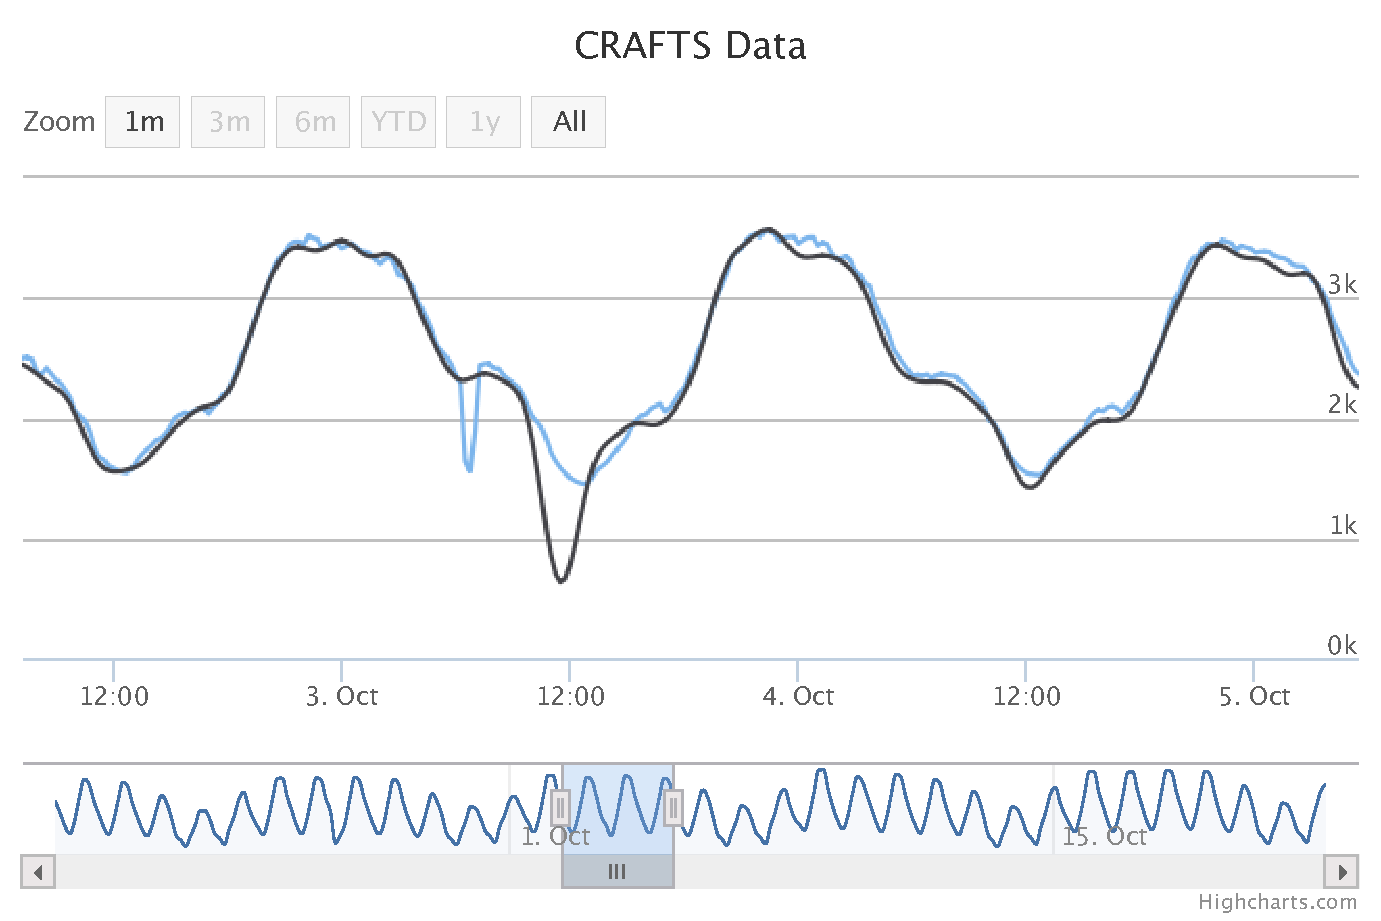
\includegraphics[width=\textwidth]{results/graphs/fft_outage.pdf}
\caption{An outage translated by the FFT predictor}
\label{fig:fft_outage}
\end{figure}

\begin{figure}
\centering
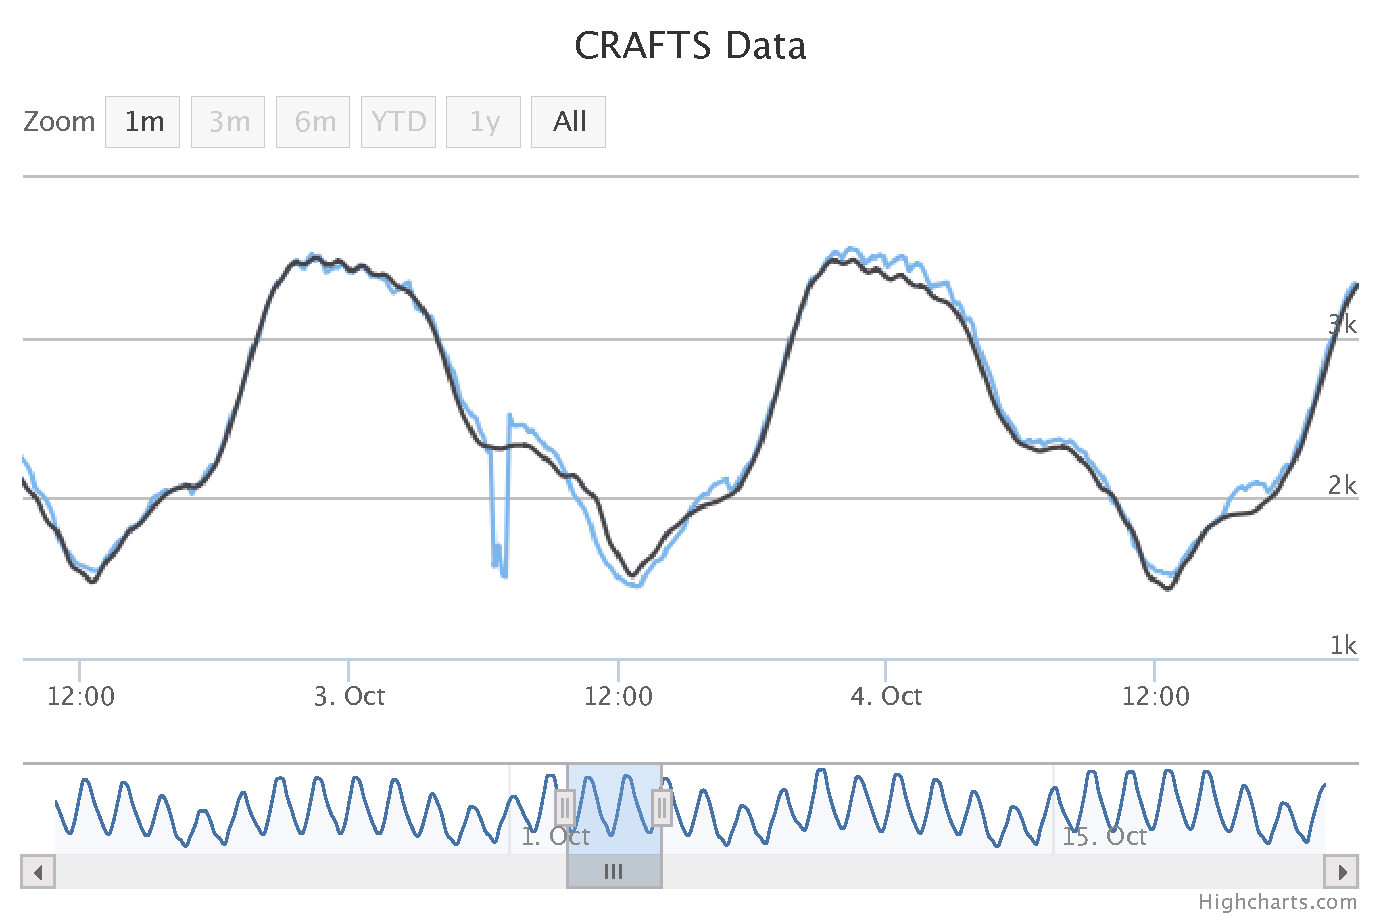
\includegraphics[width=\textwidth]{results/graphs/fft_spike.pdf}
\caption{A usage spike translated by the FFT predictor}
\label{fig:fft_spike}
\end{figure}

\begin{table}[H]
\centering
\begin{tabular}{| l | l | l |}
\hline
Type & RMSD & Percent \\ \hline
Under & 107 & 69.5\% \\ \hline
Over & 78 & 30.5\% \\ \hline
Total & 99 & \\ \hline
\end{tabular}
\caption{FFT predictor results for the baseline workload}
\end{table}

% Outage workloads

\begin{table}[H]
\centering
\begin{tabular}{| l | l | l |}
\hline
Type & RMSD & Percent \\ \hline
Under & 109 & 69.1\% \\ \hline
Over & 78 & 30.9\% \\ \hline
Total & 100 & \\ \hline
\end{tabular}
\caption{FFT predictor results for the 10-minute outage workload}
\end{table}

\begin{table}[H]
\centering
\begin{tabular}{| l | l | l |}
\hline
Type & RMSD & Percent \\ \hline
Under & 116 & 67.6\% \\ \hline
Over & 77 & 32.4\% \\ \hline
Total & 105 & \\ \hline
\end{tabular}
\caption{FFT predictor results for the 30-minute outage workload}
\end{table}

\begin{table}[H]
\centering
\begin{tabular}{| l | l | l |}
\hline
Type & RMSD & Percent \\ \hline
Under & 127 & 67.9\% \\ \hline
Over & 78 & 32.1\% \\ \hline
Total & 114 & \\ \hline
\end{tabular}
\caption{FFT predictor results for the 60-minute outage workload}
\end{table}

% Spike workloads

\begin{table}[H]
\centering
\begin{tabular}{| l | l | l |}
\hline
Type & RMSD & Percent \\ \hline
Under & 108 & 68.8\% \\ \hline
Over & 77 & 31.2\% \\ \hline
Total & 99 & \\ \hline
\end{tabular}
\caption{FFT predictor results for the low spike workload}
\end{table}

\begin{table}[H]
\centering
\begin{tabular}{| l | l | l |}
\hline
Type & RMSD & Percent \\ \hline
Under & 108 & 68.8\% \\ \hline
Over & 78 & 31.2\% \\ \hline
Total & 99 & \\ \hline
\end{tabular}
\caption{FFT predictor results for the mid spike workload}
\end{table}

\begin{table}[H]
\centering
\begin{tabular}{| l | l | l |}
\hline
Type & RMSD & Percent \\ \hline
Under & 108 & 68.7\% \\ \hline
Over & 79 & 31.3\% \\ \hline
Total & 100 & \\ \hline
\end{tabular}
\caption{FFT predictor results for the high spike workload}
\end{table}